%!TEX root = ../Main.tex

\begin{figure*}[ht!]
\begin{center}
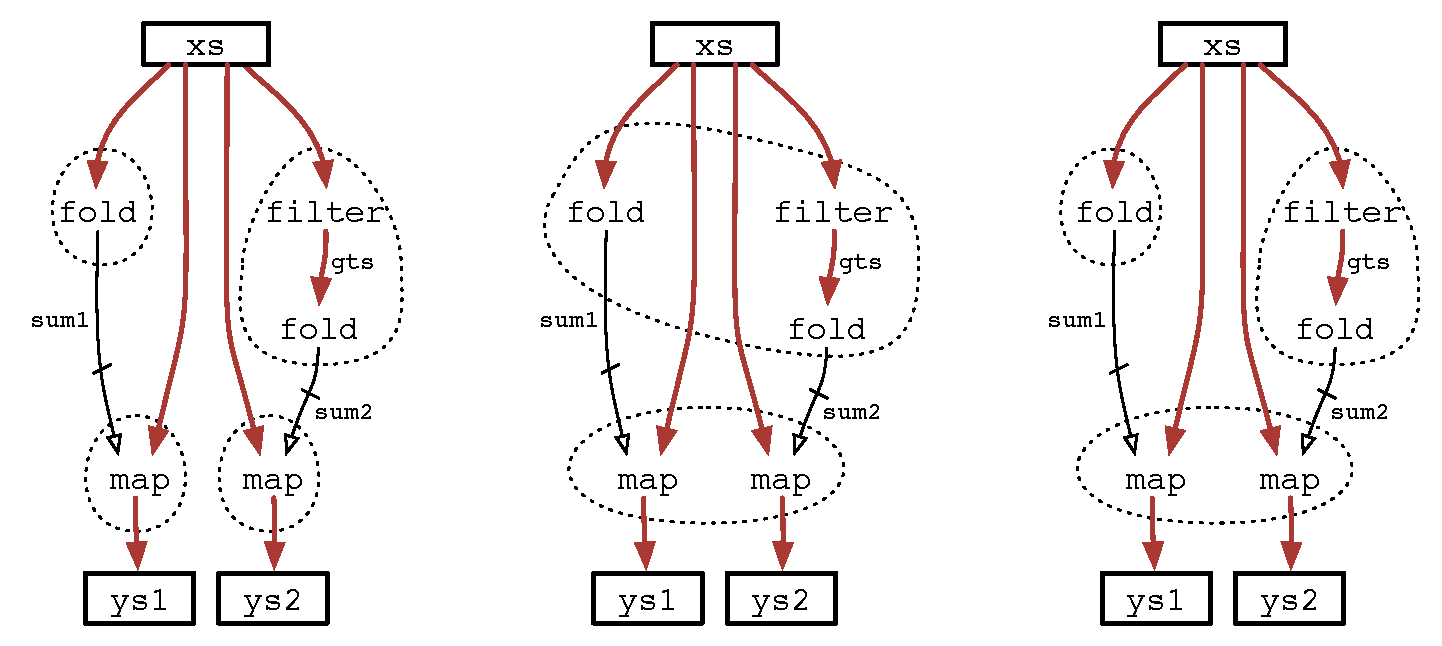
\includegraphics[scale=0.5]{figures/ex1-compare.pdf}
\end{center}
\caption{Clusterings for normalize2 example: with stream fusion; our system; best imperative system}
\label{f:normalize2-clusterings}
\end{figure*}


% -----------------------------------------------------------------------------
\section{Combinator Normal Form}
Each input program is expressed in \emph{Combinator Normal Form} (CNF), which is a textual description of its data flow graph. The grammar for CNF is in Figure~\ref{f:CombinatorNormalForm}. Both the @normalize@ and @normalize2@ examples on the previous page are in CNF, and the matching data flow graph for @normalize2@ is in Figure~\ref{f:normalize2-clusterings}. Our data flow graphs are similar to Loop Communication Graphs (LCGs) from related work in imperative array fusion \CITE. We name edges after the corresponding variable from the CNF form, and edges which are fusion preventing are drawn with a dash through them (as per the edge labeled @sum1@ in Figure~\ref{f:normalize2-clusterings}). In data flow graphs we tend to elide the worker functions to combinators when they are not important to the discussion --- so we don't show the @(+)@ operator on each use of @fold@.

Once we have determined how the operators in a data flow graph should be clustered, we highlight materialized array variables by drawing them in boxes. In Figure~\ref{f:normalize2-clusterings}, the variables @xs@, @ys1@ and @ys2@ are always in boxes as these are the material input and output arrays of the program. However, in the graph on the far right hand side @gts@ has also been materialized because in this version the producing and consuming operators (@filter@ and @fold@) have not been fused.

In Figure~\ref{f:CombinatorNormalForm} note that the bindings have been split into the ones that produce scalar values ($sbind$), and the ones that produce array values ($abind$), and these groupings are represented as open and closed arrow-heads in Figure~\ref{f:normalize2-clusterings}.

Most of our array combinators are standard, and suggestive types are given at the bottom of Figure~\ref{f:CombinatorNormalForm}. The $@map@_n$ combinator takes a worker function, $n$ arrays of the same length, and applies the worker function to all elements at the same index. As such it is similar to Haskell's @zipWith@, except for the length restriction on the argument arrays. The @generate@ combinator takes an array length and a worker function, and creates a new array by applying the worker to each index. The @gather@ combinator takes an array of elements, an array of indices, and produces the array of elements that were at each index. In Haskell this would be @gather arr ixs = map (index arr) ixs@. The @cross@ combinator returns the cartesian product of two arrays. 

The exact form of the worker functions is left unspecified, as it is not important for the discussion. We assume workers are pure, can at least compute arithmetic functions of their scalar arguments, and index into arrays in the environment. We assume that each CNF program considered for fusion is embedded in a larger ``host program'' which handles file IO and the like. Workers are additionally restricted so they can only directly reference the \emph{scalar} variables bound by the local CNF program, though they may reference array variables bound by the host program. All access to locally bound array variables is via the formal parameters of array combinators, which ensures that all data dependencies we need to consider for fusion are explicit in the data flow graph.

The @external@ binding invokes a host library function that can produce and consume arrays, but not be fused with other combinators. All arrays passed to, and returned from host functions are full materialised. External bindings are explicit \emph{fusion barriers}, which force arrays and scalars to be fully computed before continuing. 

% When the function computed is the identity, they can also be used to force a particular intermediate array to be materialized, which provides the programmer fine-grained control over exactly what clustering is produced by our algorithm.

%!TEX root = ../Main.tex
\begin{figure}
\begin{tabbing}
MMMM        \= MM \= MMMMMMMMM \= \kill
$scalar$    \> $\to$ \> (scalar variable) \\
$array$     \> $\to$ \> (array variable)  \\
$f$         \> $\to$ \> (worker function) \\
$fun$       \> $\to$ \> $f~scalar\ldots$
\\[2ex]
$bind$      \> @::=@ \> $scalar$ \> $=~sbind$ \\
            \> $~|$  \> $array$  \> $=~abind$ \\
            \> $~|$  \> $scalar\ldots,array\ldots$ \> $=~@external@~scalar\ldots~array\ldots$
\end{tabbing}

\begin{tabbing}
MMMM        \= MM \= MMMMM \= MMMMMM \= M \= MMMM \= MMMMMM \= \kill
$sbind$     \> @::=@ \> $@fold@$     \> $fun~~ array$
\\[1ex]

$abind$     \> @::=@ \> $@map@_n$    \> $fun~~ array^n$ 
            \> $~|$  \> $@filter@$   \> $fun~~ array$   \\
            \> $~|$  \> $@generate@$ \> $scalar~~ fun$  
            \> $~|$  \> $@gather@$   \> $array~~ array$ \\
            \> $~|$  \> $@cross@$    \> $array~~ array$
\\[1ex]
$function$  \> @::=@ \> $\lambda scalar\ldots~array\ldots~\to$ \\
            \>          \> $@let@~bind\ldots$                  \\
            \>          \> $@in@~(scalar\ldots,~array\ldots)$
\\[3ex]
$@fold@$     \> $:~ (a \to a \to a) \to @Array@~~ a \to a$     \\
$@map@_n$    \> $:~ (\{a_i          \to\}^{\;i\; \gets 1 \dots n}~~ b)  \to
                       \{@Array@~~ a_i \to\}^{\;i\; \gets 1 \dots n}~~ @Array@~~ b$ \\
$@filter@$   \> $:~ (a \to @Bool@) \to @Array@~~ a \to @Array@~~ a$      \\
$@generate@$ \> ~~ $:~ @Nat@ \to (@Nat@ \to a) \to @Array@~~ a$          \\
$@gather@$   \> ~~ $:~ @Array@~~ a \to @Array@~~ @Nat@  \to @Array@~~ a$ \\
$@cross@$    \> ~~ $:~ @Array@~~ a \to @Array@~~ a ~~~~ \to @Array@~~ a$
\end{tabbing}
\caption{Combinator normal form}
\label{f:CombinatorNormalForm}
\end{figure}



